%!TEX root =./Thesis.tex

\chapter{Vector vortex beam recognition}
\label{chapter:ML_VVBs}

\tmpHeading{Summary of the chapter}
In this chapter we present a method to classify experimental states with nontrivial orbital angular momentum structure using~\acf{ML} techniques.
% The employed experimental apparatus is similar to the one used in~\cref{chapter:experimental_engineering_qudits}.
The goal is to classify experimentally generated states from the sole knowledge of their intensity profile as captured with a CCD camera.
For the purpose, we use \ac{ML} algorithms to characterise experimental \acfp{VVB} generated using the platform presented in~\cref{chapter:experimental_engineering_qudits}.
We will find that a range of supervised and unsupervised learning techniques are suitable to tackle this problem, and provide useful insights on the structure of experimentally produced states.
We first train \acp{CNN} to classify experimental images.
We then discuss how the joint application of \ac{DR} and \acp{SVM} can also be used to classify states, and even obtain a full description of a state from its intensity profile.
These algorithms are fully independent on the specifics of the experimental apparatus, and are thus applicable in a variety of situations.

\tmpHeading{Previous applications of ML to structured light}
As discussed in~\cref{sec:intro:ML}, \ac{ML} provides a versatile toolbox to tackle a variety of tasks arising in experimental platforms. It has, in particular, proven useful to characterise quantum protocols and dynamics~\cite{carrasquilla2019reconstructing,giordani2018experimental, agresti2019pattern,lumino2018experimental,rocchetto2019experimental,butler2018machine,fischer2006predicting,melnikov2018active,wang2017experimental}.
In the context of structured light, \acp{NN} have been used to classify \ac{OAM} states of classical light for long distance free-space communication, even in the presence of environmental turbulence~\cite{krenn2014communication,krenn2016twisted,doster2017machine,park2018demultiplexing,lohani2018turbulence,li2018joint}.

\tmpHeading{The novelty of our work}
In contrast to these previous endeavours, we deal with the classification of \acp{VVB}. Moreover, owing to the variety of techniques we deploy, we can address both classification and regression tasks, thus enabling the reconstruction of the input states in a variety of scenarios involving structured light beams.
Our findings demonstrate the reliability of a broader class of ML techniques, providing novel recognition methods to deal with \acp{VVB}, which are a building block for several information protocols with high-dimensional systems.
This approach requires neither additional interferometry stabilisation nor spatial filtering. This makes it a robust strategy to decode information stored in \acp{VVB}, and a promising pathway to manage high-dimensional quantum systems. 

\begin{figure}[tb]
	\centering
   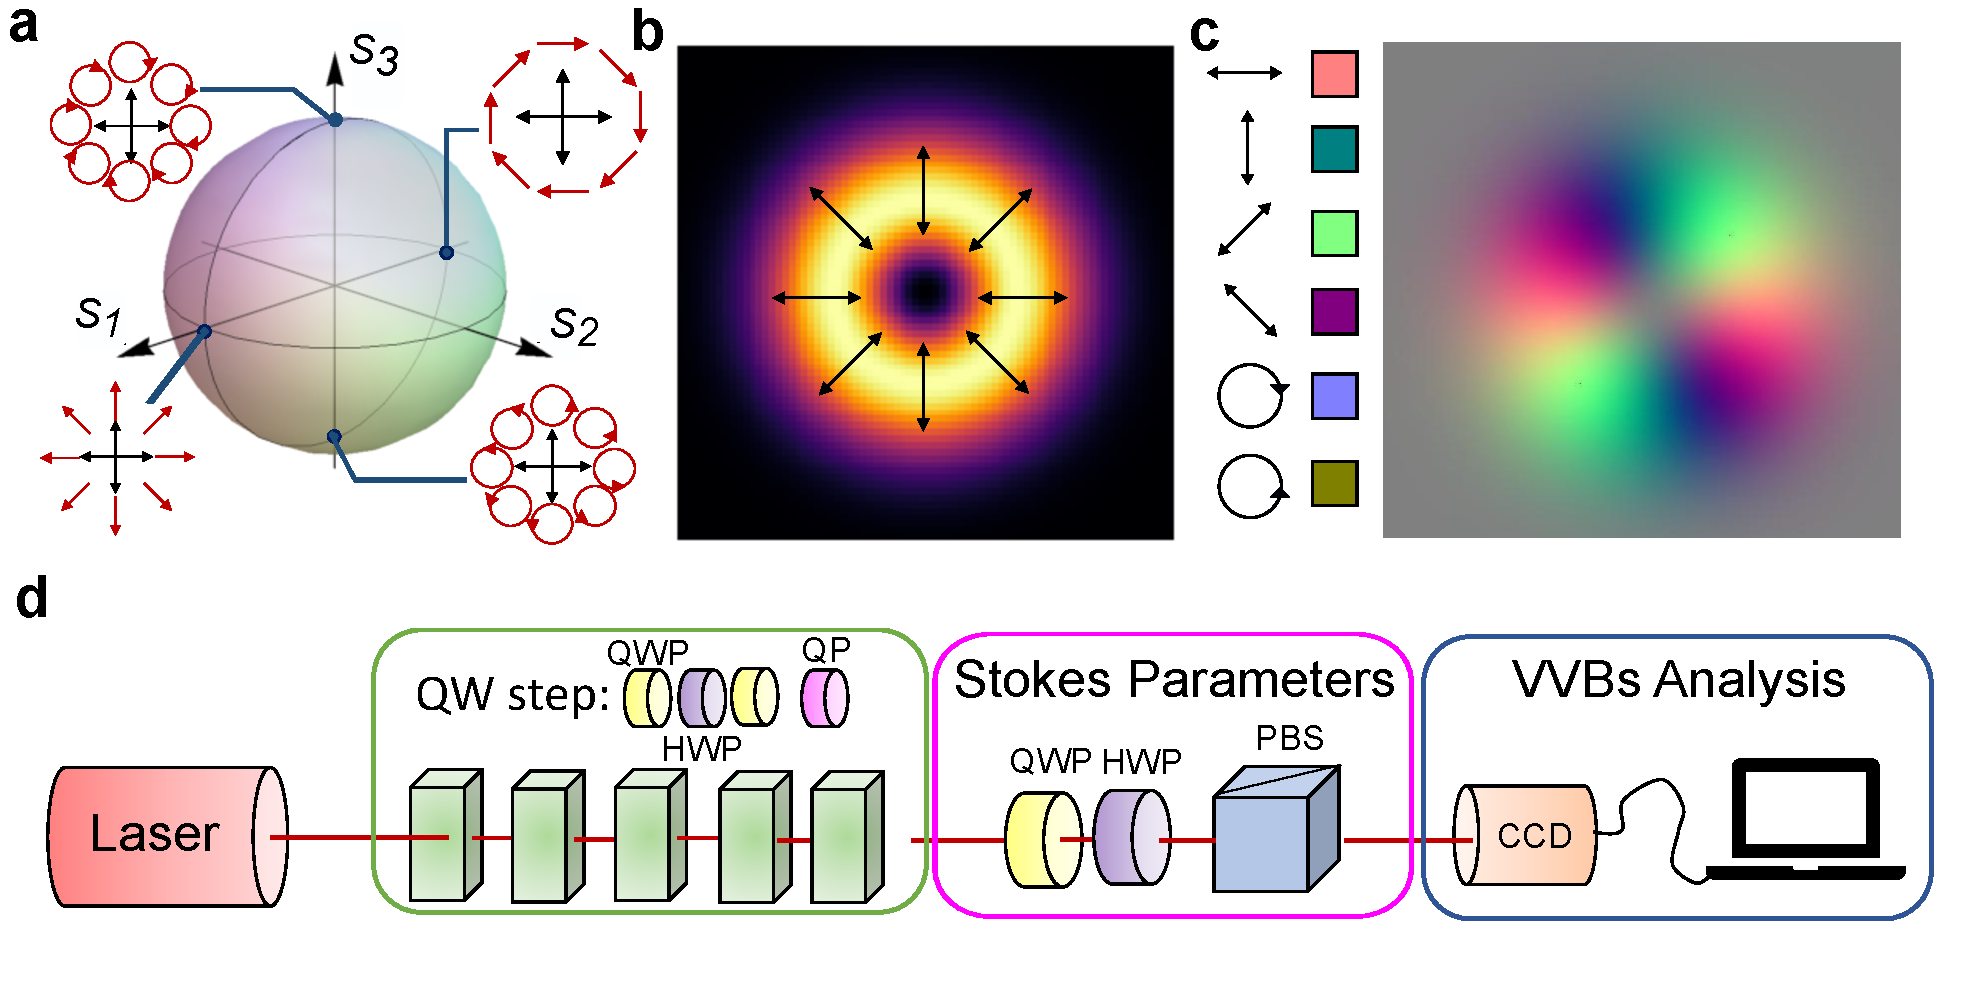
\includegraphics[width=0.8\textwidth]{VVBs-Fig1.pdf}
    \caption{
    	\textbf{(a)} High-order Poincar\'e sphere representation for $|m_{1,2}|=1$. Each point on the sphere corresponds to a VVB. 
	    \textbf{(b)} The intensity profile of a radially polarised \ac{VVB}, in which the polarisation direction always points outwards from the centre.
	    \textbf{(c)} An example of a colour-encoded VVB.
	    The legend reports the correspondence between colours and the different polarisations.
	    \textbf{(d)} Simple schematic of the experimental apparatus used to generate the \acp{VVB}. A continuous-wave laser emits a Gaussian beam $\on{TEM}_{00}$ at $\SI{808}{\nm}$. The light undergoes a $5$-step QW evolution, realised through a sequence of waveplates and QPs.
    	A CCD camera-based detection stage acquires the output intensity profiles, after projecting onto different polarisation states, thus allowing to compute the associated Stokes parameters.
    }%
    \label{fig:VVBs:poinc_sphere}
\end{figure}


\section{Experimental generation of Vector Vortex Beams}

\tmpHeading{VVBs}
\acfp{VVB} are superpositions of orthogonal polarisations states coupled with different \ac{OAM} states~\cite{padgett2004lights}.
More specifically, the electric field $\bs{E}_{m_1m_2p}$ of a \ac{VVB} decomposes as the sum of two~\ac{LG} modes with same $p$ and different azimuthal numbers $m_1>m_2$ carried by orthogonal polarisations:
\begin{equation}
	\bs{E}_{m_1m_2p} =
	\bs{e}_L \cos(\theta/2)\on{LG}_{m_1p} +
	\bs{e}_R e^{i \phi} \sin(\theta/2)\on{LG}_{m_2p},
	\label{eq:VVBs:definition_VVBs_field}
\end{equation}
where $\theta\in[0,\pi], \phi\in[0,2\pi]$ and the unit vectors $\bs{e}_{L,R}$ represent left and right circular polarisation, respectively.
For the purpose of this work we can ignore the radial number, fixing $p=0$.
For any given value of the parameters $(m_1, m_2, \theta, \phi)$, the polarisation pattern of a \ac{VVB} can be represented as a point in a \emph{generalised Poincar\'e sphere}, as also shown in~\cref{fig:VVBs:poinc_sphere}.
% In particular, we use the higher-order Poincar\'e representation in which the poles represent eigenstates of the total angular momentum but with opposite signs~\cite{milione2011higherorder}.
Each VVB can be characterised via its \emph{Stokes parameters} $(S_1,S_2,S_3)$.
These are defined in terms of the output intensities associated to different polarisation measurements.
Projecting the polarisation onto the three standard mutually unbiased bases, $b_1=(H,V), b_2=(D,A), b_3=(L,R)$, and denoting the two intensities corresponding to a given basis $b_j$ with $(I_{b_j,1},I_{b_j,2})$, the Stokes parameters are defined as
\begin{equation}
	S_{b_j} = \frac{I_{b_j,1}-I_{b_j,2}}{I_{b_j,1}+I_{b_j,2}}.
\end{equation}
%This is a way to characterise a state via its \emph{Stokes parameters} at every point of the transverse %profile.
%To do this, we first measure the output intensities $I_{b_j,1},I_{b_j,2}$ associated to a given choice of %polarisation basis $b_j$, and then compute the value of the corresponding Stokes parameter $S_{b_j}$ as %$S_{b_j}=(I_{b_j,1}-I_{b_j,2})/(I_{b_j,1}+I_{b_j,2})$.
%The canonical choice for the polarisation bases is $b_1=(H,V), b_2=(D,A)$ and $b_3=(L,R)$.
%%
It is worth noting that the Stokes parameters are the classical counterparts of the coordinates of density matrices in state space, upon replacement of intensities with probabilities.
In particular, for states living in a two-dimensional space, the Stokes parameters correspond to the coordinates in the Bloch sphere (which is often referred to as a \emph{Poincaré sphere} in this context).

\tmpHeading{Experimental generation and detection of VVBs}
As already discussed in~\cref{chapter:experimental_engineering_qudits}, we generate VVBs via polarisation-controlling waveplates interspersing $5$ cascaded QPs.
% This allows to generate VVBs with OAM quantum numbers taking odd values in the interval $\{-5,..,5\}$.
% Using different configurations of waveplates we can generate different VVBs.
% corresponding to different pairs $(m_1,m_2)$ of OAM quantum numbers, and parameters $(\theta, \phi)$.
The OAM azimuthal quantum numbers accessible with this scheme correspond to the walker states accessible via a $5$-step QW, that is, $\pm1,\pm3$, and $\pm5$.
Generated VVBs are characterised by the values of the three Stokes parameters at each point of their transverse profile. This amounts to collecting six intensities per pixel. The detection is carried out with a \ac{CCD} camera with resolution $1360 \times 1024$. 
We find, however, that a resolution of $128 \times 128$ is already sufficient for the tasks we consider, and the training stages are significantly sped up by reducing the resolution of the images (and thus the dimensionality of the handled data). We coarse-grain the images by integrating sub-matrices of the appropriate dimensions.

\tmpHeading{Colour-encoding VVBs}
To represent visually VVBs' polarisation patterns, we use a Red-Green-Blue (RGB) colour encoding, mapping each $S_j$ into the strength of one of the primary colours.
More precisely, for each pixel of the CCD, the value of the red channel is set to $255\times(S_1+1)/2$, so that the red channel is saturated when $S_1=1$ and empty when $S_1=-1$ (remembering that $S_i\in[-1,1]$). Green and blue channels are defined similarly with $S_2$ and $S_3$.
An example of such colour encoding is given in~\cref{fig:VVBs:poinc_sphere}.
These images can also be understood as vectors of length $3\times M$ with $M$ the total number of pixels supported by the CCD camera. These vectors are what the ML algorithms use.

\begin{figure}[tb]
	\centering
	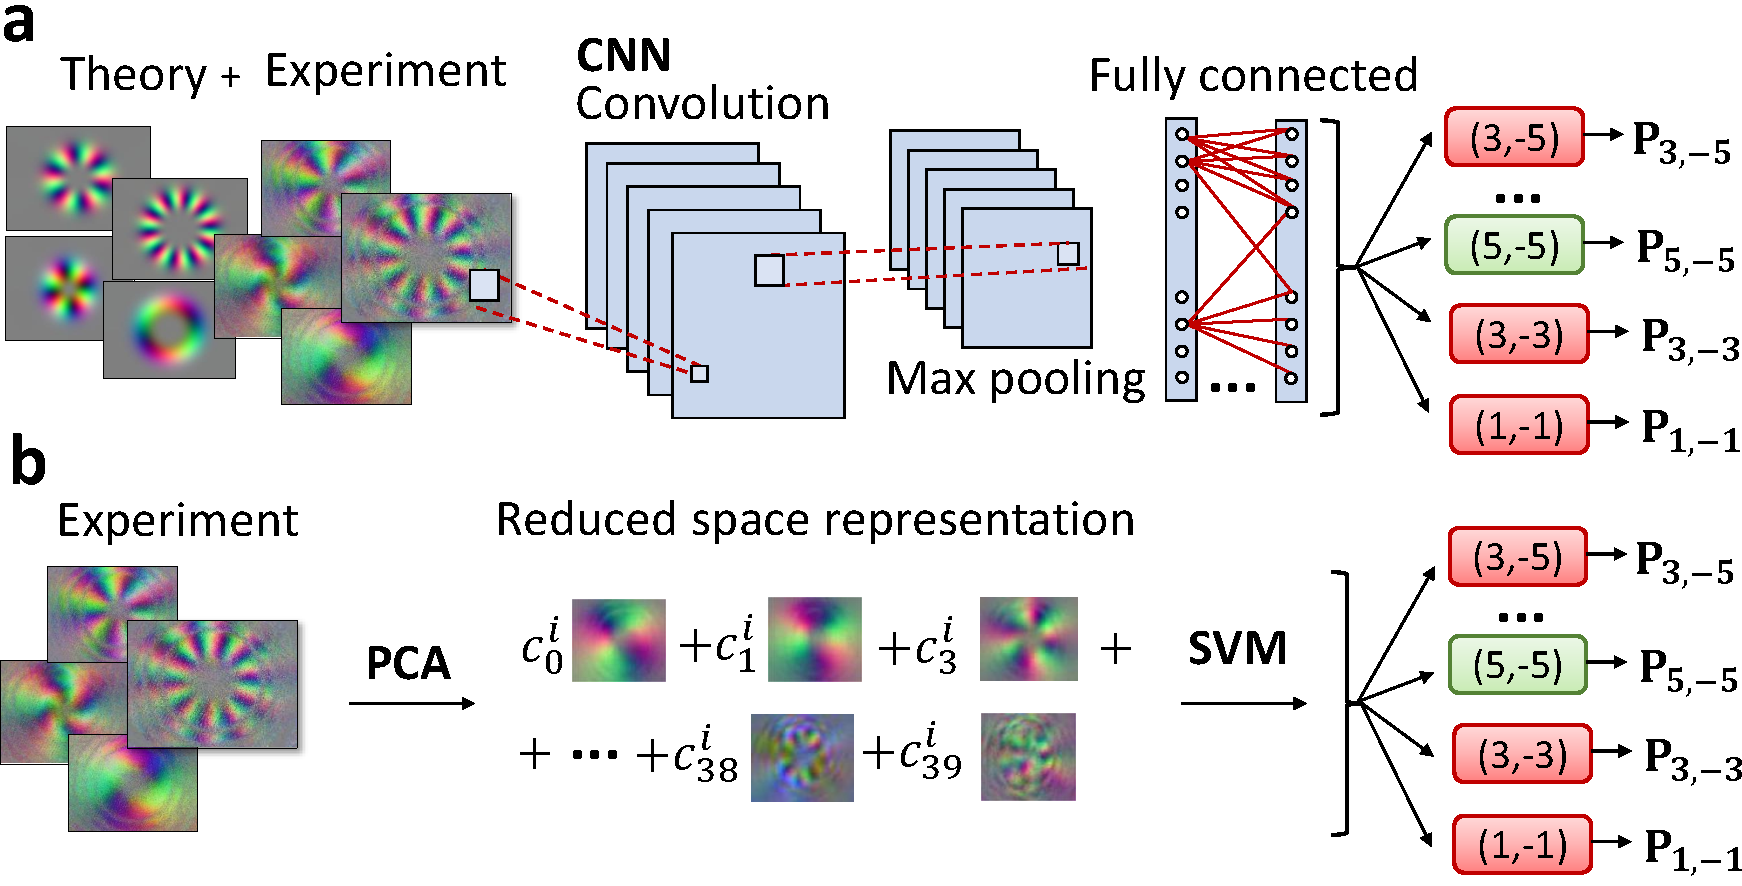
\includegraphics[width=\textwidth]{conc_VVB_2.pdf}
	\caption{
	\textbf{(a)}
	Working principles of \acp{CNN}. The training set consists of a series of simulated images, plus some others collected from the experimental platform.
	\textbf{(b)}
	Classification scheme using linear \ac{PCA}.
	After reducing the dimensionality of the dataset via \ac{PCA}, a linear \ac{SVM} is used to classify experimental images. 
	}
	\label{fig:VVBs:class_techniques}
\end{figure}

\begin{figure}[tb]
    \centering
    \includegraphics[width=0.7\textwidth]{VVBs-Fig3.pdf}
    \caption{
	    \textbf{(a)} Comparison between expected and recorded polarisation patterns for some \acp{VVB} of the ensemble in table, with the corresponding values $(m_1,m_2)$.
	    \textbf{(b)} Scaling of the average accuracy per class when classifying states into one of the $15$ VVB classes,
	    against the fraction of experimental images in the training set. 
	    Inset: best truth table.
	    Rows (columns) stand for the possible $(m_1,m_2)$ pairs (as assigned by the CNN). The matrix elements have been averaged over $100$ experimental images per class.
    }%
    \label{fig:VVBs:resultsCNN}
\end{figure}



\section{Convolutional neural networks}
\label{sec:VVBs:CNNs}

\tmpHeading{What do we use CNNs for?}
We showcase the potential of \acp{CNN} to retrieve a description of the states generating a given experimental dataset.
In particular, we test CNNs on two separate classification tasks.
First, we train a CNN to find the OAM numbers $(m_1,m_2)$ corresponding to input VVB images. Then, assuming a dataset produced using only VVBs with fixed $(m_1,m_2)$, we train a CNN to find the values of $(\theta,\phi)$ for each VVB.

\tmpHeading{What are CNNs?}
\acp{CNN} are translation-invariant deep NNs designed to handle image classification tasks~\cite{lecun2015deep}. Among their countless applications, CNNs have been used to recognise off-centre images and segmented handwritten digits~\cite{simard2003best,ciresan2011flexible},
and for facial recognition tasks~\cite{matsugu2003subject}.
In its simplest form, a \ac{CNN} consists of a \emph{convolutional layer},
 % which consists of a series of nonlinear transformations applied to the input images,
followed by a \emph{max-pooling layer}, and finally a \emph{fully connected layer}.
These build up a mapping from each image to one of an element of a finite set of outputs (the \emph{classes} defining the problem under consideration, which in our case would be the $(m_1,m_2)$ pairs).
% , categorising the information extracted in the previous layers into one of a small number of possible output categories.
\begin{itemize}
	\item (\textbf{\emph{Convolutional layer}})
		The idea of the convolutional layer is to extract local features from the image.
		This is done by computing the inner product of every $k\times k$ block of the image with a fixed $k\times k$ matrix, which in this context is called a \emph{filter}. The filter is applied sequentially to each $k\times k$ block, starting from one corner and moving at discrete steps. The size of these steps is known as the \emph{stride}.
		Each such filter extracts a specific type of feature from the image. The output of this process is called a \emph{feature map}. Multiple filters, and thus multiple feature maps, can be applied to the same image, to extract different features.
		The filters are randomly initialised, and then adjusted during the training via a standard back-propagation process.
		A nonlinear function is then applied to the feature maps. A common choice is mapping each pixel into a binary value. This nonlinearity is crucial, lest the whole process be linear and thus unable to capture interesting features.
	\item (\textbf{\emph{Pooling layer}})
		After convolution and nonlinearity follows a \emph{max pooling} stage. Here, the feature maps are down-sampled, for example by subdividing each feature map into $\ell\times \ell$ blocks, and mapping each such block into its average value.
		This is used to filter out the most relevant features from the feature maps, thus reducing noise and increasing the efficiency of training.
	\item (\textbf{\emph{Fully connected layer}})
		Finally, a fully connected layer is applied to the output of the max-pooling stage, mapping its output to one of the different classes defining the problem.
		This stage operates like a standard NN layer.
		This is the layer at which the final decision is reached: based on the activations of the final neurons in this layer, the network takes a decision as to which class the input belongs to (for example by choosing the neuron with the largest activation).
\end{itemize}
Note that most CNNs will not actually follow this simple structure, but rather contain different numbers of convolutional, pooling, and fully connected layers in different arrangements and with different parameters, depending on the specific applications.

\tmpHeading{Categorisation into discrete classes}
We first feed the network with a training dataset of simulated images of \acp{VVB}. The goal is to classify states in $15$ classes, each one defined by a pair of OAM numbers $(m_1,m_2)$, as per~\cref{fig:VVBs:resultsCNN}\textbf{a}.
For each class we generate states with $\theta=\pi/2$ and $\phi\in[0,2\pi]$. The size of the training set is $400$ images per class.
% Additional $100$ simulated images per class are used to benchmark the performance during training. In these conditions, the network achieves an accuracy of $100\%$.
We then collect $100$ experimental images per class, to use as test set.
To test the effectiveness of using simulated images to classify experimental ones, we add different fractions of experimental images into the training dataset.
\Cref{fig:VVBs:resultsCNN}{\bf a}-{\bf b} shows the mean accuracy per class against the fraction of experimental images added to the training dataset.
Remarkably, a small increase of the number of experimental images in the training set results in a good accuracy reached by the network: $12.5\%$ is already sufficient to achieve an average accuracy of $\sim 0.989$.


\tmpHeading{Retrieving the position in the Poincaré sphere}
We also test the network on a different problem: assuming $(m_1,m_2)$ is fixed, retrieve the parameters $(\theta,\phi)$ characterising the VVB (remembering the definition of VVBs as given in~\cref{eq:VVBs:definition_VVBs_field}).
In particular, we train a CNN to retrieve the values $(\theta,\phi)$ characterising VVBs corresponding to the OAM quantum numbers $m_1=-m_2=1$.
The network is thus trained to discriminate both rotations in the polarisation patterns (corresponding to changes of $\phi$), and variations in the colour tone (corresponding to changes of $\theta$).
To frame this as a classification task, we partition the sphere in $26$ disjoint sectors.
Working in spherical coordinates, we partition $\theta$ is in the $3$ intervals $\left[k \frac{\pi}{8}, (k+2) \frac{\pi}{8}\right]$ with $k=1,3,5$, and $\phi$ in the $8$ intervals $\left[t \frac{\pi}{4}, (t+1) \frac{\pi}{4}\right]$ with $t \in \{0,...,7\}$.
This leaves two classes surrounding the two poles of the sphere, corresponding to $\theta \in \left[0, \frac{\pi}{8}\right]$ and $\theta\in\left[ \frac{7}{8} \pi, \pi\right]$.
Partitioning makes the classification of VVBs closer to the border of two sectors harder, but nonetheless provides useful information about the suitability of CNNs for this kind of task.
We train the CNN with $500$ simulated images per class in the training set, and $125$ per class in the validation one. The maximum accuracy  achieved is $\sim 0.90$.
The suboptimality of this result can be understood as consequence of framing the problem as a classification task. Training a CNN for the corresponding regression task will potentially give much better results.

\tmpHeading{How do we implement the CNN?}
To build and train the \acp{CNN} we use the Python library \emph{Keras}~\cite{chollet2015keras}.
We use three convolutional layers) and one classifier. Each convolutional layer uses $32$ filters of size $3 \times 3 \times 3$, with a Rectified Linear Unit (ReLU) as activation function, and unit stride. The ReLU is the function $x\mapsto \max(x,0)$.
This means that, for each input image of dimension $3\times 128\times128$ (three colour channels per each pixel in the $128\times128$ grid), the $i$-th activation map contains the values obtained by computing the inner products of the $i$-th filter with each $3\times 3$ contiguous block of the image. Each filter potentially acts differently on the different colour channels, so that, effectively, each colour map is the results of using three $3\times3$ filters (one per colour channel) on the three channels of the image.
Explicitly, we write each input image as a three-index tensor $\calI_{\alpha,ij}\equiv\calI^\alpha_{ij}$, with $\alpha=1,2,3$ the colour channels and $i,j=1,...,128$ the pixels indices.
Writing the filters as the tensor $\calF_{k\alpha mn}\equiv\calF^{k\alpha}_{mn}$, with $k=1,..,32$ indexing the different filters, we then compute the activation maps $\calM_{k\alpha pq}$ as
\begin{equation}
	\calM_{k,\alpha, p,q} = (\calF^{k\alpha}\star\calI^{\alpha})_{pq} \equiv
	\sum_{mn} \calF^{k\alpha}_{mn} \calI^\alpha_{R[p,q]_{mn}},
\end{equation}
where $\star$ denotes the $2$D convolution operation, which consists in computing the inner product of $\calI^\alpha$ with the different $3\times3$ blocks of $\calF^{k\alpha}$. To explicit the convolution operation, we denoted with $R[p,q]$ the indices of a $3\times3$ block corresponding to the indices $p,q$.
Explicitly, $R[p,q]_{mn}\equiv (p+m-2,q+n-2)$, so that for example $R[1,1]$ covers the $3\times3$ submatrix surrounding the $(1,1)$ element of the image (which is the upper-left pixel). Whenever $R[p,q]$ covers pixels that fall outside of the boundaries of the image, like is the case for $R[1,1]$, it is standard practice to apply some \emph{padding} to the image, which in this case amounts to adding a single row or column of zeros on each side of the image. This is done to avoid having the bordering pixels being given a lesser weight than the rest.
Once the activation maps are computed, the ReLU activation function is applied element-wise to $\calM_{k,\alpha, p,q}$.
This process is also illustrated with an explicit example in~\cref{fig:VVBs:convolutions_example}.
The pooling layer acts on the previously computed activation maps by reducing the number of parameters. In particular, the $\max$ function is applied to every $2\times2$ block of the previous layers' output, meaning that every such block is sent to its greatest element.
The classification is finally performed by a fully connected layer which uses a sigmoid activation function. The network training consists of a finite number of epochs, each of which is composed of $200$ training steps and $100$ validation steps.

% channel1 = ConstantArray[0, {7, 7}];
% channel1[[2 ;; 6, 2 ;; 6]] = RandomInteger[{0, 2}, {5, 5}];
% channel2 = ConstantArray[0, {7, 7}];
% channel2[[2 ;; 6, 2 ;; 6]] = RandomInteger[{0, 2}, {5, 5}];
% channel3 = ConstantArray[0, {7, 7}];
% channel3[[2 ;; 6, 2 ;; 6]] = RandomInteger[{0, 2}, {5, 5}];

% filter1 = RandomInteger[{-1, 1}, {3, 3}];
% filter2 = RandomInteger[{-1, 1}, {3, 3}];
% filter3 = RandomInteger[{-1, 1}, {3, 3}];

% grayBorderingSquares[size_Integer] := {LightGray,
%      Rectangle[{#1, #2} - 0.45, {#1, #2} + 0.45] &[##]
%      } & @@@ Select[
%     Tuples[Range@size, {2}],
%     Min@# == 1 || Max@# == size &
%     ];
% greenInsideSquares[size_Integer] := {LightGreen,
%      Rectangle[{#1, #2} - 0.45, {#1, #2} + 0.45] &[##]
%      } & @@@ Select[
%     Tuples[Range@7, {2}],
%     Min@# > 1 && Max@# < size &
%     ];
% squaresGrid[xs_, ys_, color_] := {color,
%    Rectangle[{#[[1]], #[[2]]} - 0.45, {#[[1]], #[[2]]} + 0.45] & /@ 
%     Tuples@{xs, ys}
%    };

% numbersInMatrix[matrix_] := Table[
%    Text[matrix[[Dimensions[matrix][[2]] + 1 - j, i]], {i, j}],
%    {i, 1, Dimensions[matrix][[1]]}, {j, 1, Dimensions[matrix][[2]]}
%    ];

% tripleCopy[expr_, size_] := 
%   Translate[expr, {0, #}] & /@ {0, -size - 1, -2 size - 2};

% fig = With[{size = Length@channel1}, Graphics[{
%     {grayBorderingSquares@size, greenInsideSquares@size} // 
%      tripleCopy[#, size] &,
%     Translate[numbersInMatrix@#[[1]], {0, #[[2]]}] & /@ Thread@{
%        {channel1, channel2, channel3}, {0, -size - 1, -2 size - 2}
%        }
%     (*{FaceForm[],EdgeForm[{Thick,Red}],Rectangle[{#2,
%     size+1-#1}-0.45,{#2,size+1-#1}+0.45]&[1,3]}*)
%     , 
%     tripleCopy[#, size] &@
%      {FaceForm[], EdgeForm[{Thickness@0.01, Red}], 
%       Rectangle[{5, 5} - 0.48, {7, 7} + 0.45] &[1, 3]},
%     Sequence @@ With[{xmin = 7, xmax = 12.5},
%       tripleCopy[#, size] &@
%        {Thick, Dashed, Red,
%         {Line@{{xmin, 4.5}, {xmax, 4.5}}},
%         {Line@{{xmin, 7.5}, {xmax, 7.5}}},
%         {Line@{{xmax - 3, 4.5}, {xmax - 3, 7.5}}},
%         {Line@{{xmax, 4.5}, {xmax, 7.5}}}}
%       ],
%     squaresGrid[Range[10, 12], Range[5, 7], LightRed] // 
%      tripleCopy[#, size] &,
%     Translate[numbersInMatrix[filter1], {9, 4}],
%     Translate[numbersInMatrix[filter2], {9, 4 - size - 1}],
%     Translate[numbersInMatrix[filter3], {9, 4 - 2 size - 2}],
%     Arrow@{{13, 6}, {15, 6}} // tripleCopy[#, size] &,
%     {FaceForm[], EdgeForm[{Black, Thick, Dashed}], 
%       Rectangle[{16, 6} - 0.5, {16, 6} + 0.5]} // 
%      tripleCopy[#, size] &,
%     Text[Style[
%       Total[Flatten@channel1[[;; 3, 5 ;; 7]]*Flatten@filter1], 
%       Bold], {16, 6}],
%     Text[Style[
%       Total[Flatten@channel2[[;; 3, 5 ;; 7]]*Flatten@filter2], 
%       Bold], {16, 6 - size - 1}],
%     Text[Style[
%       Total[Flatten@channel3[[;; 3, 5 ;; 7]]*Flatten@filter3], 
%       Bold], {16, 6 - 2 size - 2}]
%     }, ImageSize -> 300]]

\begin{figure}[tb]
    \centering
    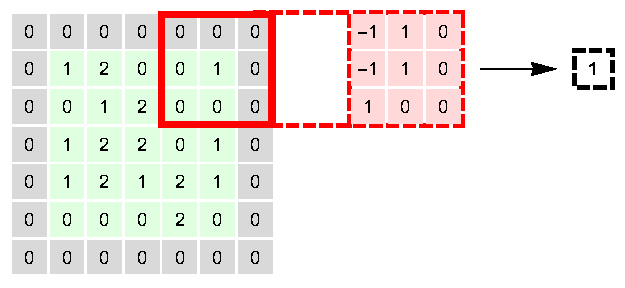
\includegraphics[width=0.5\linewidth]{VVBs-CNNconvolutions-scheme-1row}
    \caption{
    	Simple illustration of how a filter is applied to an input image.
    	The green square represents an input image, focussing on a single channel. In our notation, assuming the first channel, this would be $(\calI^1_{ij})_{ij}$ with $i,j=1,...,5$.
    	The gray squares represent the padding applied to the image.
    	The dashed red square is a $3\times 3$ filter, which is here shown applied to the upper-right $3\times3$ block of the image.
    	In our notation, the filter is $\calF^{1,1}$ (assuming $k=1$ for the first filter). The thick red square is $R[1,5]$. The dashed black rectangle on the right contains the result of computing the inner product of the filter with the highlighted block of the image.
    	Being the result $1>0$, the ReLU nonlinearity leaves it unchanged.
    }%
    \label{fig:VVBs:convolutions_example}
\end{figure}


\section{Dimensionality reduction}
\label{sec:VVBs:dimensionality_reduction}

\tmpHeading{A different approach to classify images}
While CNNs provide good performance for general image classification tasks, the specific structure of the datasets we deal with can be leveraged to make for more efficient algorithms. In particular, we know that the datasets consist of intensity patterns associated with (mostly pure) quantum states.
% we can hope to achieve similar performances in the tasks we are interested in by exploiting additional structure that we know is intrinsic to our dataset, due to it consisting of a set of intensities associated with states of light.
In this section we present alternative approaches to extract information the dataset of interest, using \ac{DR} to expose the intrinsic structure of the dataset.


\tmpHeading{DR and PCA}
\acf{DR} is a class of algorithms whose goal is to find low-dimensional encodings of high-dimensional datasets~\cite{cunningham2008dimension,fodor2002survey}.
This has several applications, from data visualisation, to improving the efficiency of classification and regression algorithms, which can be applied on the reduced representation of the data.
A classical \ac{DR} algorithm is \acf{PCA}.
In its simplest form, \ac{PCA} is a \emph{linear} \ac{DR} algorithm which, given a dataset of vectors in a high-dimensional space $\RR^n$, finds the directions which capture the maximum amount of information about the dataset~\cite{jolliffe2011principal,jolliffe2016principal}.
More specifically, given a dataset comprised of $N$ real vectors of length $M$, we define the \emph{data matrix} $\bs X$ as the $N\times M$ matrix whose $i$-th row is the $i$-th dataset vector. \ac{PCA} then finds the vectors $\bs a\in\RR^{M}$ that maximise the variance of $\bs X\bs a$. This turns out to be equivalent to diagonalising $\bs S\equiv \tilde{\bs X}^T\tilde{\bs X}/(N-1)$, where $\tilde{\bs X}$ is the \emph{centered data matrix}, which is equal to $\bs X$ modulo each of its columns shifted in order to average to zero.
The first $k$ \emph{principal components} found by \ac{PCA} are then the $k$ eigenvectors of $\bs S$ corresponding to the largest $k$ eigenvalues.
Note that these principal components are themselves vectors of the same ``type'' as the data vectors. This means that \ac{PCA} effectively generates a set of data vectors which ``optimally represent'' the information content of the given dataset.

\tmpHeading{PCA and VVBs}
The rationale behind using \ac{PCA} in the context of \acp{VVB} is that, although experimental images live in extremely high-dimensional spaces (whose dimension is of the order of the number of pixels of the \ac{CCD} camera), the underlying dimension of the generated \acp{VVB} is typically much lower.
This means that, although the experimental dataset might \emph{a priori} seem like a complicated bundle of high-dimensional vectors, the underlying data is actually characterizable by a small number of parameters.
% Furthermore, the linearity of the mapping from the full to the reduced space makes it preserve many of its geometrical properties.
This is a form of \emph{unsupervised} learning, in that we gain useful information about the the images without feeding the algorithm with any prior knowledge about their structure.


% \tmpHeading{For example...}
% For example, in our case, each row of $\bs X$ is a vector of length $128\times128\times3$ containing the Stokes parameters $S_{b_1}, S_{b_2}, S_{b_3}$ for each pixel of the camera.
% Because each image corresponds to such a vector, and vice versa each such vector corresponds to the image of a \ac{VVB}, we can represent the principal components found by \ac{PCA} again in the form of images, which allows us to gain some intuition into the type of principal components that optimally represent the data according to \ac{PCA}.


\subsection{Retrieving states from probabilities}

\tmpHeading{Measuring in a single measurement basis}
Collecting experimental intensity images with the \ac{CCD} camera is akin to collecting the statistics resulting from a specific state measured in a fixed measurement basis.
In general, this is not sufficient to fully reconstruct the corresponding state, but in specific circumstances it is possible to obtain a full description of a state from the results in a single measurement basis~\cite{banchi2018multiphoton}.
More specifically, let $\rho$ be the density matrix characterising the state. The corresponding observed statistics in a chosen measurement basis is given by the set of probabilities
\begin{equation}
	p_k = (\calU\rho\calU^\dagger)_{kk}
	    = \sum_{ij}\calU_{ki}\bar\calU_{kj}\rho_{ij},
\end{equation}
for some unitary $\calU$.
This means that the mapping between density matrices and detected probabilities is linear: $\bs p=\Psi(\rho)$ for some linear map $\Psi$. This implies that many geometrical features of the space of states is preserved in the probabilities space. Moreover, a suitable choice of $\Psi$ will allow to retrieve $\rho$ from the knowledge of $\bs p$.
For this to be possible, $\Psi$ needs to have a number of rows greater than or equal to the number of columns. Physically, this amounts to the measurement basis containing a sufficient number of elements. More specifically, $\Psi$ needs to be \emph{left-invertible}, which is the case when its columns are linearly independent.


\tmpHeading{Application to experimental VVB images}
In our case, $\rho$ is a description of a VVB in the OAM-polarisation basis, while $\calU$ is the unitary mapping this basis into the position basis, which is the one that CCD cameras naturally operate on. In principle, one might need to take care of the different dimensionalities of these two spaces (the OAM space is countable while the position one is not), but this is easily fixed by discretising the position space, which is what is done naturally by the finite number of pixels of the CCD camera. 
In other words, $\rho$ describes the state in the OAM-polarisation basis, which is the basis in which the generated states are efficiently described, whereas $\calU\rho\calU^\dagger$ describes the same state in the position basis, which is the one in which the CCD camera operates on.
The set of detected probabilities is then given by $\bs p=\on{diag}(\calU\rho\calU^\dagger)\equiv\Psi(\rho)$,
where $\Psi$ is defined as the linear map that sends $\rho$ to the set of measured probabilities $\bs p$.
It should be noted that, while here we use a formalism and vocabulary evocative of quantum states, the states actually used in the experiment are classical. This in no way impacts the formal description of the protocol, and the only thing that should change when the states used are classical is that the probabilities $\bs p$ should be reinterpreted as intensities.
Crucially, the linearity of $\Psi$ implies that it preserves the \emph{convexity} of the space of states, and therefore many of its geometrical features.
For example, if we consider the set of states of the form $c_0 \ket{\uparrow,m=m_1} + c_1 \ket{\downarrow,m=m_2}$ with $m_1\neq m_2$, then the associated density matrices will be arranged to form a three-dimensional sphere embedded in the full state space (because these are effectively different states of a single qubit).
Thanks to the linearity of $\Psi$, \emph{the corresponding probabilities $\bs p$ will also be contained in a spherical surface}, up to possible rescaling of the axes.
In other words, the Bloch sphere of the original two-dimensional system is still present, albeit hidden, in the experimental images, embedded into an extremely high-dimensional space.


\begin{figure}[tb]
    \centering
    \includegraphics[width=0.8\linewidth]{VVBs-Fig4.pdf}
    \caption{
		\textbf{(a)} High order Poincar\'e sphere for \acp{VVB} with $|m_{1,2}|=1$. Magenta-coloured parallels (Blue-coloured meridians) mark intervals between consecutive values of $\theta$ ($\phi$). 
		Along a meridian the colours of the pattern vary from the hottest to the coldest one. Along a parallel, the patterns rotate. 
		\textbf{(b)}
		Comparison between experimental and simulated \ac{VVB} images for different angles $(\theta, \phi)$.
		\textbf{(c)}
		Distribution of fidelities obtained comparing each experimental VVBs with its reduced 3D representations given by PCA. Projecting each image onto its first three principal axes and rescaling brings the data (orange points) onto a sphere in 3D, as shown in the inset. The inner (outer) black (semi-transparent) sphere is added for contrast [radius equal to that of the point with smaller (larger) radius].
		\textbf{(d)}
		Average prediction accuracy of a linear \ac{SVM} classifier, trained and tested after applying linear DR to the data, against the number of reduced dimensions $n_c$.
		For each of the 15 classes (cf.~\cref{fig:VVBs:resultsCNN}a) in which the experimental dataset was divided, we show in the inset the true-table. 
    }%
    \label{fig:VVBs:PCAresults}
\end{figure}


\subsection{Results}

\tmpHeading{PCA applied to experimental data}
As a notable example, we apply these observations to VVBs with $m_2=-m_1=1$, which can be pictured as lying on a sphere, in the higher-order Poincaré representation. 
of the form $c_0 \ket{L,m=1} + c_1 \ket{R, m=-1}$ with $\abs{c_0}^2+|c_1|^2=1$.
The inclusion of only two orthogonal basis states makes these states effectively equivalent to a single qubit. 
Indeed, \ac{PCA} applied to the experimental dataset of~\cref{fig:VVBs:PCAresults}\textbf{b}, 
reveals that only three directions capture most of the information content of the images. Projecting the images along these three principal components, we recover that the data is arranged in the form of a three-dimensional sphere embedded in the high-dimensional space of experimental (cf. inset of~\cref{fig:VVBs:PCAresults}\textbf{c}).
Remarkably, this was not obvious from the experimental dataset alone, but was easily found via \ac{DR}. This result highlights the potential of \ac{DR} to  reveal features of the underlying states generating a given experimental dataset, also in the presence of experimental noisy conditions.
To assess the accuracy of such reconstruction, we compute the average fidelity $\mathcal F_{\text{avg}}$ between the expected state and the one found by our analysis with PCA. As shown in the histogram of Fig.~\ref{fig:VVBs:PCAresults}c,  this is found to be $\mathcal F_{\text{avg}}\sim0.96$ (standard deviation $\sim0.01$), thus certifying the quality of the reconstruction.

\begin{figure}[tb]
  \centering
  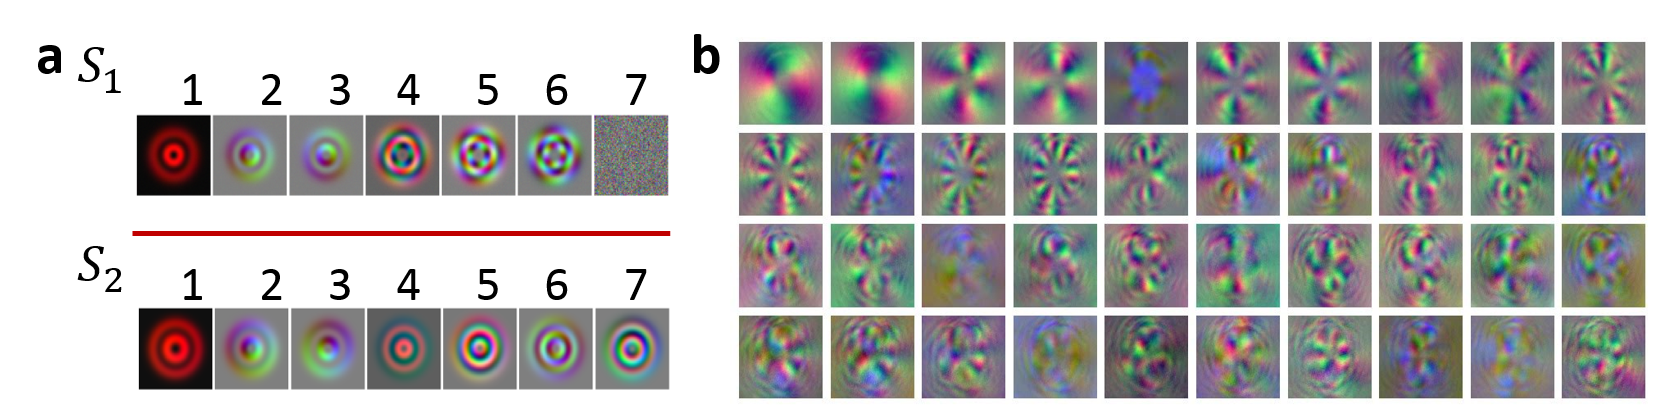
\includegraphics[width=0.98\textwidth]{S1_fig.png}
  \caption{
      \textbf{a,}
       Principal components obtained using PCA on simulated datasets of noisy VVB. The first (second) row shows the first seven principal components obtained on the dataset $\mathcal S_1$ ($\mathcal S_2$). 
       The first 6 (all 7) components correspond to non-vanishing singular values.
       \textbf{b,} First 40 principal components individuated in the experimental dataset corresponding to the 15 classes labelled by $(m_1,m_2)$, discussed in the main text.%
    }
    \label{fig:S1}
\end{figure}


\tmpHeading{Toy examples of application of PCA to VVBs}
To see the usefulness of these ideas to understand the type of states generated by a given apparatus, we consider here two examples of applications of \ac{PCA} for different types of input states. 
In all of these cases, \ac{PCA} is applied without any previous knowledge of the type of states that underly the observed experimental images, and is therefore to be considered a type of \emph{unsupervised learning}.
Consider a simulated set of images corresponding to VVBs of the form
$c_1\ket{L,m=1}+c_2\ket{R,m=2}$ and
$c_1\ket{L,m=1}+c_2\ket{R,m=4}$, where the coefficients $c_i$ are sampled uniformly at random from the set of $c_{1},c_2\in\mathbb{C}$  such that $|c_1|^2+|c_2|^2=1$ (\emph{i.e.} uniformly sampled on the Bloch sphere).
Applying PCA to this dataset, we find six non-vanishing singular values, whose associated principal components are given in Fig.~\ref{fig:S1}a.
This is consistent with the dimension of the subspace  spanned by states of the form $\mathcal S_1=\{c_1\ket{L,1}+c_2\ket{R,2}, c_3\ket{L,1}+c_4\ket{R,4}\}$,  as the set of corresponding density matrices is spanned by the six orthogonal matrices
$X^{(1,2)}, X^{(1,4)}, Y^{(1,2)},Y^{(1,4)},Z^{(1,2)}\pm Z^{(1,4)}$, where $X^{(i,j)}=\ketbra{i}{j}+\ketbra{j}{i}$ is the Pauli $X$ matrix acting on the $(i,j)$ subspace, and similarly for $Y^{(i,j)}$ and $Z^{(i,j)}$.
On the other hand, if the dataset under consideration consists of states of the form $\mathcal S_2=\{c_1\ket{L,1}+c_2\ket{R,2}, c_3\ket{L,3}+c_4\ket{R,4}\}$, then \ac{PCA} finds \emph{seven} principal components associated with non-vanishing singular values (see Fig.~\ref{fig:S1}a).
This is consistent with the underlying state space being spanned by the seven orthogonal Hermitians:
\begin{equation}
\begin{gathered}
    X^{(1,2)}, \,\, X^{(3,4)}, \,\,
    Y^{(1,2)}, \,\, Y^{(3,4)}, \\
    Z^{(1,2)},\quad
    -Z^{(1,2)} + 2 Z^{(1,3)}, \\
    -Z^{(1,2)} - Z^{(1,3)} + 3 Z^{(1,4)}.
\end{gathered}
\end{equation}
These matrices can be obtained by direct analysis of the type of states contained in $\mathcal S_2$ and then finding a set of orthogonal Hermitian matrices generating the corresponding set of density matrices.
It is worth noting how this method provides a quick and easy way to gain useful information about the dimensionality of generated states, as well as about other properties such as specific symmetries, which, as shown in~\cref{fig:S1}, are often picked up by the principal components.


\section{Support vector machines}
\label{sec:VVBs:SVMs}

\subsection{What are they?}

\tmpHeading{What are SVMs?}
\acfp{SVM} are a class of \emph{supervised learning} algorithms, whose goal is to classify data by finding an optimal partition of the feature space such that all the vectors with the same training label lie on the same classification sector.
In particular, \emph{linear} \acp{SVM} try to separate the data linearly, that is, look for an optimal separating hyperplane.

\tmpHeading{The math of linear SVMs}
A SVM takes as input a training set of labelled data of the form $\{(\bs x_1,\ell_1),...,(\bs x_n,\ell_n)\}$ where $\bs x_i\in\RR^N$ and $\ell_i$ is one of two possible labels, $N\in\NN$ being here the dimension of the feature vectors. If there are only two possible labels, we can conventionally assume $\ell_i\in\{-1,1\}$.
The goal is to find a linear separation, which is characterised by two parameters $\bs w$ and $b$ which identify an hyperplane as the set of $\bs x\in\RR^N$ such that $\bs w\cdot\bs x=\bs b$. We want this hyperplane to be such that, for all training vectors $\bs x_i$, the constraint $\ell_i(\bs w\cdot\bs x_i-\bs b)\ge1$ is satisfied.
New data is then categorised using the \emph{classifier} $g_{\bs w,\bs b}(\bs x)=2\Theta(\bs w\cdot\bs x-\bs b)-1$, which equals $\pm1$ depending on whether the point $\bs x$ is on one side or the other of the separation determined by $\bs w,\bs b$.
This is the so-called \emph{hard-margin} SVM, because this is only possible if every single training point is strictly on one or the other side of the separating hyperplane.
An often more practical alternative are the so-called \emph{soft-margin} SVMs, in which this strict requirement is lifted. Instead, the goal becomes to minimise the average value of
$\max(0, 1- \ell_i (\bs w\cdot\bs x_i-\bs b))$, trying at the same time to keep $\|\bs w\|$ as low as possible. This variation makes the algorithm more robust and able to classify data even in the presence of some noise \highlight{(an example with figures of hard- vs soft-margin classification would be nice)}.


\subsection{How do we use them?}

\tmpHeading{SVMs after PCA}
We now show how the reduced representations provided by \ac{PCA} can function as starting point to train a classifier with an accuracy comparable with that of the \acp{CNN} used in~\cref{sec:VVBs:CNNs}, whilst requiring a drastically reduced amount of computational resources.
More precisely, we use as classifiers linear multiclass \acp{SVM}~\cite{hearst1998support,shawe2000support}. These supervised learning algorithms categorise data by finding the hyperplane that optimally separates the training dataset in accordance with the corresponding labels.
We use here in particular a \emph{linear}, multiclass \ac{SVM}, whose goal is to find hyperplanes in the feature space that optimally separate the datapoints corresponding to different classes.
During the training phase, a set of training experimental images is used to find the separating hyperplanes, which is then used to classify new experimental images.
% Both training and classification are performed \emph{after} the dimensionality reduction has been carried out via \ac{PCA}. This makes for improved computational times as well as making the algorithm more robust to experimental noise and imperfections.

\tmpHeading{What do we use the SVMs for?}
As done for the \ac{CNN}, we consider the task of classifying experimental dataset of VVBs. We train a \ac{SVM} on the reduced space obtained via \ac{PCA}, applied to the experimental dataset reported in~\cref{fig:VVBs:resultsCNN}\textbf{a}. This stage significantly improves the training cost of the classifier since the latter will work on a synthesised description of the high-dimensional space of images in which the features of each class can be easily recognised.
This not only significantly speeds up the training stage, but also makes for a more robust classification, thanks to the property of dimensionality reduction algorithms to weed out statistical and experimental noise.
What's more, the geometrical picture offered by the reduced representation tells us when we should expect this classification to be accurate: \ac{PCA} effectively retrieves the description of the states in the generalised Bloch representation, therefore the classification will give good results whenever the states are linearly separated in state space.


\tmpHeading{What is used for the training?}
The~\ac{SVM} was trained on half of the experimental data, with the other half used to test the resulting accuracy. A breakdown of the classification performance is reported in the inset of~\cref{fig:VVBs:PCAresults}\textbf{d}, where we detail how the images belonging to each class were classified.

\tmpHeading{What kind of SVM do we use?}
We used here a \emph{linear} SVM, instead of a commonly used SVM with RBF kernel, because we found it to perform better: an RBF kernel was found to give, in our case, an average accuracy of only $\sim94\%$.
Furthermore, in~\cref{fig:VVBs:PCAresults}\textbf{d} we highlight how the average overall accuracy depends on the dimension of the reduced representation: $\sim 25$ dimensions are already sufficient to get good average accuracies.

\subsection{Results}

The average classification accuracy achieved on images not included in the training set is $\sim 98 \%$. This result confirms that the description provided by \ac{PCA} is sufficient to capture the important features of the generated states, thus allowing for a dramatically more efficient classification scheme.


\section{Conclusions}
\label{sec:VVBs:conclusions}

We presented a new approach to classify \acp{VVB} leveraging ML techniques. We demonstrated how the use of inference strategies based on CNNs and PCA (enhanced by SVMs) allows to extract efficiently properties of high-dimensional photonic \ac{VVB} systems.
In particular, DR was used to obtain a deeper understanding of the underlying geometrical properties of the experimentally generated states, without requiring prior knowledge about the physics of the generation apparatus.
% this is not quite right
By embedding a variety of {\ac{ML}} algorithms into our experimental pipeline, the task of characterising structured light is made significantly broader in the methods, ranging from supervised to unsupervised learning, and more flexible in the applications, classification and regression tasks.
%
%Then, the investigation of different techniques in the ML field has provided a more general framework for the characterization of structured light. 
% 
While paving the way to further experimental validations -- potentially also in experimental settings that do not rely on optical networks -- we believe that numerous tasks of relevance to modern photonics could benefit from introducing similar {\ac{ML}} ideas into their characterisation protocols. These techniques can prove to be useful add-on to tasks ranging from the design of automatised approaches to the characterisation of experimental platforms and experiments, to the provision of solutions to OAM demultiplexing in the context of classical and quantum communication and, more generally, for the use of structured light in quantum technologies.

\textit{Note--} During the reviewing process of this manuscript, the authors
became aware of a related work~\cite{liu2019superhighresolution} addressing a similar topic.


\tmpHeading{How do we use ML?}
% We leverage both supervised and unsupervised learning techniques.
We start by training a \ac{CNN} to classify experimental images belonging to predefined classes of states. This method gives good prediction accuracy, while remaining fairly problem-agnostic and thus useful for diverse applications. However, while providing high prediction accuracy, NN-based methods are difficult to interpret.
We thus also propose an alternative technique based on the joint application of \ac{DR} and supervised learning.
This method provides a geometrical description of the underlying space associated to the experimental data.
While significantly easier to use, such approach gives comparable results to CNN,
at the cost of being more tailored to the specifics of the problem.
